\begin{surferPage}[216奇異點]{帶有更多實奇異點的曲面}
如前所述,七次曲面上具體的最大奇異點數$\mu(7)$是不知道的。我們僅僅有一個下界和上界:$99\le \mu(7) \le 104$。對一般的次數$d$的曲面我們知之甚少。至少,松加·布萊斯克(Sonja Breske)、奧利弗·萊布斯(Oliver Labs)以及杜克·范·斯特芬(Duco van Straten)利用了奇穆托夫的一個構造使得當今最大奇異點數也能夠在帶實奇異點的曲面上實現。
至今,我們知道如下結果\[0,41\bar{6}d^3 \lessapprox \mu(d) \lessapprox 0.44\bar{4} d^3.\]
從上可知,我們可以看到此構造的對稱性以及與黑胞腔極大數目間的關係。
 \begin{center}
      \begin{tabular}{c@{\qquad}c}
        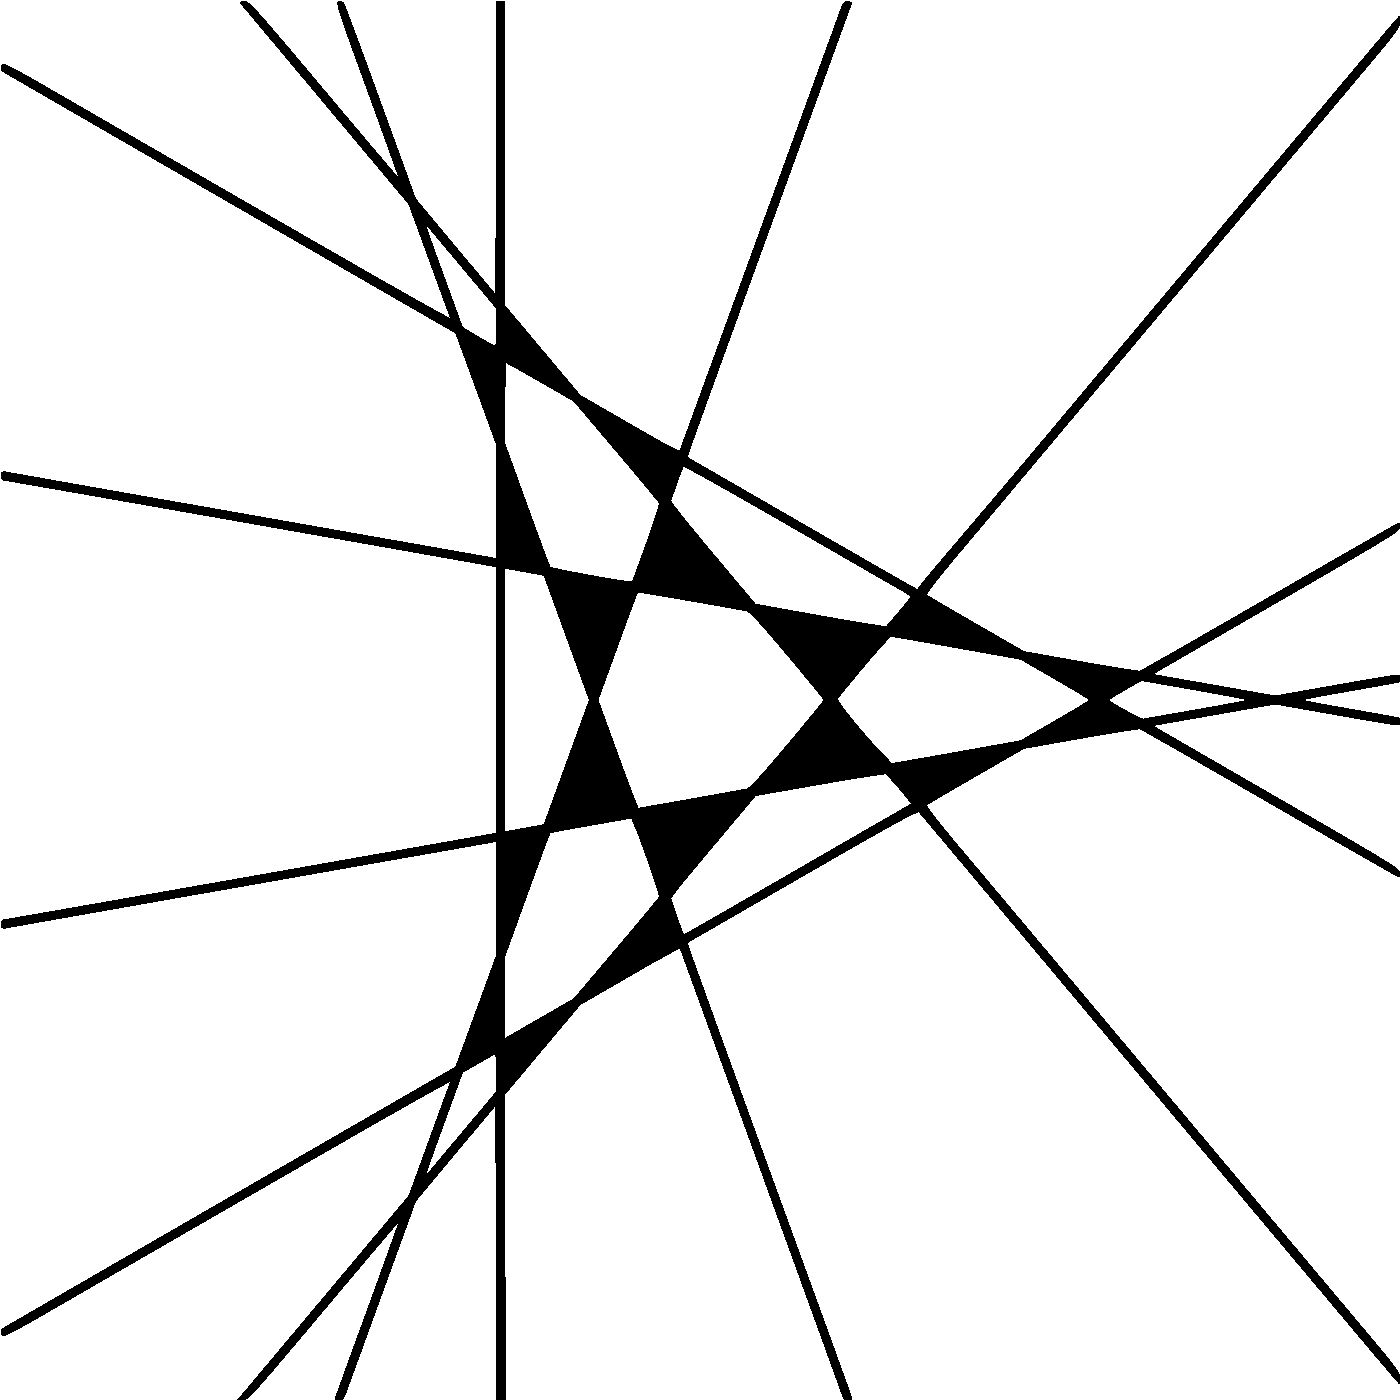
\includegraphics[height=1.5cm]{./../../common/images/vielesing.pdf}
        &
        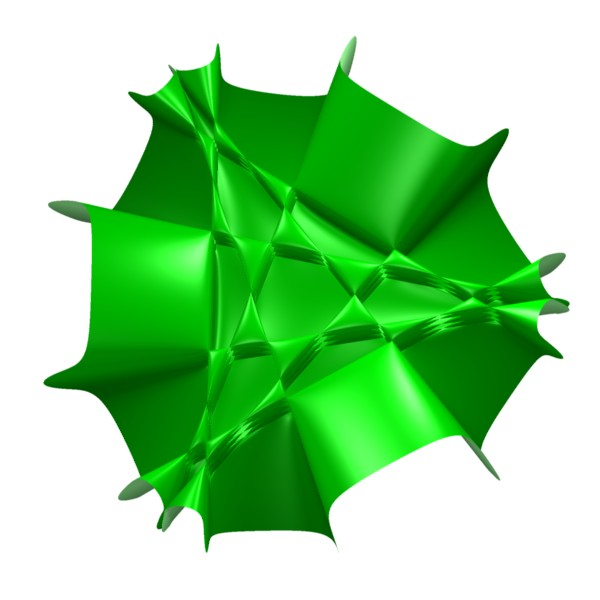
\includegraphics[height=1.5cm]{./../../common/images/p9surface_von_oben}
      \end{tabular}
    \end{center}
\end{surferPage}
